\documentclass[11pt,a4paper]{article}

\usepackage[utf8]{inputenc}
\usepackage[T1]{fontenc}
\usepackage[a4paper,margin=0.8in]{geometry}
\usepackage{array}
\usepackage{booktabs}
\usepackage{tabularx}
\usepackage{longtable}
\usepackage{pgfplots}
\usepackage{xcolor}
\usepackage{hyperref}
\usepackage{listings}
\usepackage{titlesec}

\pgfplotsset{compat=1.18}

\hypersetup{
  colorlinks=true,
  linkcolor=blue,
  urlcolor=blue
}

\definecolor{softgray}{RGB}{246,246,246}
\definecolor{okgreen}{RGB}{34,139,34}
\definecolor{warnorange}{RGB}{210,120,30}
\definecolor{softblue}{RGB}{35,92,170}
\definecolor{codegray}{RGB}{245,245,245}

\lstset{
  basicstyle=\ttfamily\small,
  backgroundcolor=\color{codegray},
  frame=single,
  breaklines=true,
  columns=fullflexible
}

\titleformat{\section}{\large\bfseries\color{softblue}}{\thesection.}{0.5em}{}
\titleformat{\subsection}{\normalsize\bfseries}{\thesubsection.}{0.5em}{}

\newcolumntype{Y}{>{\raggedright\arraybackslash}X}

\title{Wait Less\\April 10 Slide Assets Pack}
\author{Sapienza IoT Project Team}
\date{April 9, 2026}

\begin{document}

\maketitle

\noindent This PDF is a presentation-support handout. It collects the exact tables, numbers, and charts that can be copied directly into the April 10 slides.

\section{Checkpoint Message}

\begin{quote}
\textbf{Main message for the presentation:} We already validated the adaptive controller in software and validated node-to-node LoRa communication on real hardware. The remaining work is mainly sensor calibration, actuator integration, and full end-to-end validation.
\end{quote}

\section{Optional Technical Slide: Code Structure And Implementation Approach}

\begin{table}[h!]
\centering
\footnotesize
\renewcommand{\arraystretch}{1.08}
\begin{tabularx}{\textwidth}{>{\bfseries}p{0.36\textwidth} Y}
\toprule
Module or file group & Responsibility in the system \\
\midrule
\texttt{firmware/node\_a/main.cpp} & Reads side A sensors, builds telemetry, supports emulation and debug commands, and transmits compact LoRa packets. \\
\texttt{firmware/node\_b/main.cpp} & Reads side B sensors, receives Node A telemetry, runs the controller, drives the traffic-light LEDs, and reports hardware status. \\
\texttt{lib/traffic\_control/}\\\texttt{TrafficTypes.h} & Defines the shared data model: telemetry, light outputs, and controller decisions. \\
\texttt{lib/traffic\_control/}\\\texttt{AdaptiveController.*} & Contains the phase logic: minimum green, maximum green, yellow transition, demand comparison, and emergency priority handling. \\
\texttt{lib/traffic\_control/}\\\texttt{SensorSupport.*} & Isolates low-level ultrasonic reading and threshold-based occupancy detection. \\
\texttt{lib/traffic\_control/}\\\texttt{NodeMessaging.*} & Encodes and decodes the compact telemetry format exchanged between the two nodes. \\
\texttt{lib/traffic\_control/}\\\texttt{DebugSupport.h} & Provides structured log modes and report commands so testing stays readable and repeatable. \\
\bottomrule
\end{tabularx}
\caption{Code structure ready to use in a slide about implementation organization.}
\end{table}

\begin{table}[h!]
\centering
\small
\begin{tabularx}{\textwidth}{>{\bfseries}p{0.12\textwidth} Y}
\toprule
Step & Implementation approach used in the project \\
\midrule
1 & Read raw ultrasonic distances on each node and convert them into far/near occupancy states using explicit thresholds. \\
2 & Estimate queue state from sensor events rather than switching directly on a single binary trigger. \\
3 & Keep the embedded logic shared in reusable library files so the simulator and firmware follow the same policy. \\
4 & Make Node A a thin sensing and telemetry node, and keep Node B as the control and actuation node. \\
5 & Exchange a compact payload over LoRa instead of sending large or cloud-dependent messages. \\
6 & Decide switching locally on Node B using measurable timing rules: minimum green, yellow, and maximum green. \\
7 & Add structured debug and report modes so each experiment can be repeated and documented clearly. \\
\bottomrule
\end{tabularx}
\caption{Implementation approach to explain how the code was written and why it is modular.}
\end{table}

\subsection*{Short script to say on this slide}

\begin{quote}
We wrote the code in layers so that each responsibility is isolated. Sensor reading is separated from queue estimation, messaging is separated from control logic, and the shared controller sits in reusable library files. This made it possible to test the policy first in software, then reuse the same logic in the ESP32 firmware, and finally validate the communication path on real boards.
\end{quote}

\clearpage

\section{Slide 2: Baseline Requirements}

\begin{table}[h!]
\centering
\small
\begin{tabularx}{\textwidth}{>{\bfseries}p{0.10\textwidth} Y >{\raggedright\arraybackslash}p{0.14\textwidth}}
\toprule
ID & Requirement & Current value \\
\midrule
R1 & Each side is represented by two ultrasonic detections: one far and one near. & 2 detections per side \\
R2 & The controller evaluates traffic demand periodically. & 200 ms \\
R3 & Node A produces periodic telemetry for Node B. & 1000 ms \\
R4 & The controller does not switch before a minimum green interval. & 5000 ms \\
R5 & Every switch includes a yellow safety interval. & 2000 ms \\
R6 & Starvation is limited by a maximum green cap if the other side remains waiting. & 20000 ms \\
R7 & Switching is demand-based rather than purely fixed-cycle. & Score = 3 * queue + 2 * farOccupied + 4 * nearOccupied \\
\bottomrule
\end{tabularx}
\caption{Checkpoint requirements derived from the current implementation baseline.}
\end{table}

\begin{table}[h!]
\centering
\small
\begin{tabularx}{\textwidth}{>{\bfseries}Y >{\raggedright\arraybackslash}p{0.16\textwidth} Y}
\toprule
Baseline parameter & Current value & Use in the talk \\
\midrule
Control loop interval & 200 ms & State this as the current controller reaction baseline. \\
Telemetry period & 1000 ms & State this as the remote-data freshness baseline. \\
Far threshold & 35 cm & State this as the current approach-detection threshold. \\
Near threshold & 18 cm & State this as the current stop-line occupancy threshold. \\
Minimum green & 5000 ms & State this as the anti-oscillation rule. \\
Yellow interval & 2000 ms & State this as the safety transition rule. \\
Maximum green & 20000 ms & State this as the anti-starvation rule. \\
Switching margin & 4 points & State this as the current comparison threshold between sides. \\
Telemetry example & A,1,0,4,2,2,0,12345 & Use this to show the packet format. \\
Payload size & 19 bytes & Use this to show communication compactness. \\
\bottomrule
\end{tabularx}
\caption{Exact baseline numbers to place in the requirement slide.}
\end{table}

\clearpage

\section{Slide 3: Metrics Table}

\small
\begin{longtable}{>{\raggedright\arraybackslash}p{0.24\textwidth} >{\raggedright\arraybackslash}p{0.18\textwidth} >{\raggedright\arraybackslash}p{0.16\textwidth} >{\raggedright\arraybackslash}p{0.28\textwidth}}
\toprule
\textbf{Metric} & \textbf{Current value} & \textbf{Source} & \textbf{Why it matters} \\
\midrule
\endfirsthead
\toprule
\textbf{Metric} & \textbf{Current value} & \textbf{Source} & \textbf{Why it matters} \\
\midrule
\endhead
Control-loop period & 200 ms & ProjectConfig.h & Defines how often the controller can react to traffic changes. \\
Telemetry update period & 1000 ms & ProjectConfig.h & Defines how fresh remote traffic data is when Node B decides. \\
Far ultrasonic threshold & 35 cm & ProjectConfig.h & Baseline for detecting approaching traffic. \\
Near ultrasonic threshold & 18 cm & ProjectConfig.h & Baseline for detecting queue presence near the stop line. \\
Minimum green time & 5000 ms & ProjectConfig.h & Prevents unstable rapid switching. \\
Yellow transition time & 2000 ms & ProjectConfig.h & Enforces a safety interval before the other side can become green. \\
Maximum green time & 20000 ms & ProjectConfig.h & Prevents starvation of the waiting side. \\
Demand score formula & 3 * queue + 2 * farOccupied + 4 * nearOccupied & TrafficTypes.h and traffic\_logic.py & Explains how the controller compares both sides. \\
Example telemetry payload size & 19 bytes & NodeMessaging.cpp & Shows that node-to-node communication remains compact. \\
Real telemetry TX evidence & \texttt{tx=RADIO\_TX\_OK} & Node A monitor & Confirms live telemetry transmission on hardware. \\
Real telemetry RX evidence & \texttt{source=LORA\_RADIO}\\\texttt{stale=OFF} & Node B monitor & Confirms live telemetry reception on hardware. \\
\bottomrule
\caption{Metrics table ready to place in the verification slide.}
\end{longtable}

\begin{figure}[h!]
\centering
\begin{tikzpicture}
\begin{axis}[
  width=0.95\textwidth,
  height=0.30\textheight,
  ybar,
  bar width=18pt,
  ymin=0,
  ymax=22,
  ylabel={Seconds},
  symbolic x coords={Control loop,Telemetry,Yellow,Min green,Max green},
  xtick=data,
  xticklabel style={rotate=20,anchor=east},
  nodes near coords,
  every node near coord/.append style={font=\scriptsize},
  enlarge x limits=0.12,
  grid=major
]
\addplot[fill=softblue] coordinates {
  (Control loop,0.2)
  (Telemetry,1.0)
  (Yellow,2.0)
  (Min green,5.0)
  (Max green,20.0)
};
\end{axis}
\end{tikzpicture}
\caption{Current timing baseline used by the controller and telemetry path.}
\end{figure}

\section{Slide-Ready Technical Numbers}

\begin{table}[h!]
\centering
\small
\begin{tabularx}{\textwidth}{>{\bfseries}p{0.30\textwidth} >{\raggedright\arraybackslash}p{0.17\textwidth} Y}
\toprule
Technical quantity & Current value & Notes for the slide \\
\midrule
ESP32 board target & Heltec WiFi LoRa 32 V3 & Board used for both embedded nodes in the current prototype. \\
Microcontroller family & ESP32-S3 & Current hardware platform used by the firmware build. \\
CPU clock & 240 MHz & Board capability reported by the build environment. \\
RAM / Flash & 320 KB RAM / 8 MB Flash & Board capability reported by the build environment. \\
Serial monitor speed & 115200 bps & Current debug and bench-test serial speed. \\
Controller update interval & 200 ms & Equivalent to a 5 Hz control loop. \\
Telemetry interval & 1000 ms & Equivalent to a 1 Hz telemetry update rate. \\
Remote telemetry timeout & 3000 ms & Old remote data is discarded after this timeout. \\
LoRa carrier frequency & 868.0 MHz & Current configured regional radio setting. \\
LoRa bandwidth & 125.0 kHz & Current radio configuration. \\
LoRa spreading factor & SF7 & Current radio configuration. \\
LoRa coding rate & 4/5 & Current radio configuration. \\
LoRa output power & 14 dBm & Current transmit-power configuration. \\
Example application payload & A,1,0,4,2,2,0,12345 & Compact CSV-style telemetry packet. \\
Application payload size & 19 bytes & Size of the example telemetry payload above. \\
Derived radio bit rate & \~5.47 kbps & Approximate useful bit rate from the current LoRa settings. \\
Estimated airtime for 19-byte payload & \~51 ms & Approximate radio airtime per packet at the current settings. \\
\bottomrule
\end{tabularx}
\caption{Technical operating numbers that can be copied directly into a slide.}
\end{table}

\begin{table}[h!]
\centering
\small
\begin{tabularx}{\textwidth}{>{\bfseries}p{0.24\textwidth} >{\raggedright\arraybackslash}p{0.16\textwidth} >{\raggedright\arraybackslash}p{0.16\textwidth} Y}
\toprule
Power item & Current estimate & Power at 5 V & Status \\
\midrule
Node A average current & \~120 mA & \~0.60 W & Engineering estimate, not yet instrument-measured. \\
Node A peak current during TX & \~160 mA & \~0.80 W & Engineering estimate for brief radio-transmit peaks. \\
Node B average current & \~140 mA & \~0.70 W & Engineering estimate with controller and light-driving logic active. \\
Node B peak current with radio and LEDs & \~180 mA & \~0.90 W & Engineering estimate for brief active peaks. \\
Two-node system average & \~260 mA & \~1.30 W & Preliminary whole-system estimate for the current prototype. \\
\bottomrule
\end{tabularx}
\caption{Preliminary power-budget estimates. These values are placeholders for planning and must be replaced later by real instrument measurements.}
\end{table}

\subsection*{Safe sentence for the presentation}

\begin{quote}
\textbf{Use this wording:} The communication and timing values come from the implemented firmware configuration, while the current power numbers are preliminary engineering estimates for the prototype and will be replaced by instrument measurements in the final stage.
\end{quote}

\clearpage

\section{Slide 4: Experiments And Results}

\begin{table}[h!]
\centering
\small
\begin{tabularx}{\textwidth}{>{\bfseries}p{0.20\textwidth} Y Y Y}
\toprule
Experiment & Setup & Observed result & Conclusion \\
\midrule
Equal demand hold & Both sides have queue 2 from t = 6 s to t = 11 s. & Controller kept side A green. & Equal pressure does not trigger unnecessary switching. \\
Empty-lane yield & Side A becomes empty at t = 6 s while side B queue becomes 2. & Yellow at 6 s, side B green at 8 s. & Empty-lane detection yields at the first allowed instant. \\
Busier-side priority & Side A queue becomes 1 and side B queue becomes 4 after minimum green is already satisfied. & Yellow at 12 s in the scripted simulation baseline, and targeted test confirms 6 s to 8 s switching window after the trigger. & The busier side gets priority without skipping yellow. \\
Max-green enforcement & One side keeps demand for a long time while the other side continues waiting. & Yellow at 20 s, side B green at 22 s. & The maximum green cap prevents starvation. \\
Real LoRa A to B link & Node A transmits live telemetry and Node B listens over SX1262. & Node B changed from LORA\_STALE to LORA\_RADIO with stale=OFF and remoteQ=1. & Node-to-node communication was validated on real hardware. \\
\bottomrule
\end{tabularx}
\caption{Experiment summary table for the result slide.}
\end{table}

\begin{figure}[h!]
\centering
\begin{tikzpicture}
\begin{axis}[
  width=0.95\textwidth,
  height=0.30\textheight,
  ybar,
  bar width=14pt,
  ymin=0,
  ymax=24,
  ylabel={Seconds},
  symbolic x coords={Empty-lane yield,Busier side,Max green},
  xtick=data,
  xticklabel style={rotate=15,anchor=east},
  legend style={at={(0.5,1.12)},anchor=south,legend columns=-1},
  nodes near coords,
  every node near coord/.append style={font=\scriptsize},
  enlarge x limits=0.18,
  grid=major
]
\addplot[fill=warnorange] coordinates {
  (Empty-lane yield,6)
  (Busier side,12)
  (Max green,20)
};
\addplot[fill=okgreen] coordinates {
  (Empty-lane yield,8)
  (Busier side,14)
  (Max green,22)
};
\legend{Yellow start,New green}
\end{axis}
\end{tikzpicture}
\caption{Observed switch timing in the main checkpoint experiments.}
\end{figure}

\clearpage

\section{Slide 5: Hardware Evidence And Remaining Work}

\begin{table}[h!]
\centering
\small
\begin{tabularx}{\textwidth}{>{\bfseries}p{0.18\textwidth} >{\raggedright\arraybackslash}p{0.18\textwidth} Y >{\raggedright\arraybackslash}p{0.12\textwidth}}
\toprule
Area & Evidence & Interpretation & Status \\
\midrule
Node A build and upload & PlatformIO build and upload succeeded on the real board. & The transmitter firmware is build-valid and flashable. & \textcolor{okgreen}{DONE} \\
Node B build and upload & PlatformIO build and upload succeeded on the real board. & The receiver/controller firmware is build-valid and flashable. & \textcolor{okgreen}{DONE} \\
Node A telemetry path & Node A produced queue-changing payloads and reported tx=RADIO\_TX\_OK. & Telemetry generation and radio transmission work on hardware. & \textcolor{okgreen}{DONE} \\
LoRa communication & Node B reported source=LORA\_RADIO, stale=OFF, and remoteQ=1 from live Node A traffic. & Real A-to-B packet reception was validated. & \textcolor{okgreen}{DONE} \\
Ultrasonic sensing & Hardware integration started, but validation is not yet complete for all physical sensor paths. & Sensing remains an integration and calibration task. & \textcolor{warnorange}{IN PROGRESS} \\
Emergency override on hardware & Logic exists in firmware, but the full real-hardware path is not yet fully validated. & Feature is implemented but not yet fully demonstrated physically. & \textcolor{warnorange}{PENDING TEST} \\
\bottomrule
\end{tabularx}
\caption{Current hardware-validation status to show honestly in the last slide.}
\end{table}

\begin{table}[h!]
\centering
\small
\begin{tabularx}{\textwidth}{>{\bfseries}Y Y}
\toprule
Already done for the checkpoint & Remaining after the checkpoint \\
\midrule
Adaptive controller validated in software & Full ultrasonic validation on both sides \\
Firmware build validated on both boards & Full LED and sensing integration together \\
Firmware upload validated on both boards & Emergency override validation on the real hardware path \\
Node A telemetry path validated on real hardware & End-to-end tests with physical sensing and actuation \\
Real LoRa communication validated between Node A and Node B & Threshold tuning and calibration \\
\bottomrule
\end{tabularx}
\caption{Ready-made done-versus-remaining table for the closing slide.}
\end{table}

\section{Real Log Evidence}

\subsection*{Node A Evidence}

\begin{lstlisting}
Node A ready.
[LoRa] backend: RadioLib SX1262
A STATUS | source=SERIAL_EMU | far=OCC | near=FREE | queue=1 | in=1 | out=0 | emergency=OFF | tx=RADIO_TX_OK | payload=A,1,0,1,0,1,0,62000
A STATUS | source=SERIAL_EMU | far=FREE | near=OCC | queue=1 | in=1 | out=0 | emergency=OFF | tx=RADIO_TX_OK | payload=A,0,1,1,0,1,0,70000
A STATUS | source=SERIAL_EMU | far=FREE | near=FREE | queue=0 | in=1 | out=1 | emergency=OFF | tx=RADIO_TX_OK | payload=A,0,0,1,1,0,0,79000
\end{lstlisting}

\subsection*{Node B Evidence}

\begin{lstlisting}
Node B ready.
[LoRa] backend: RadioLib SX1262
B STATUS | far=999.0cm/FREE | near=999.0cm/FREE | localQ=0 | remoteQ=0 | source=LORA_STALE | stale=ON | green=A | phase=GREEN | emergency=OFF | priority=A | lights=A:GREEN B:RED
B STATUS | far=999.0cm/FREE | near=999.0cm/FREE | localQ=0 | remoteQ=1 | source=LORA_RADIO | stale=OFF | green=A | phase=GREEN | emergency=OFF | priority=A | lights=A:GREEN B:RED
\end{lstlisting}

\section{Sources Inside The Repository}

\begin{itemize}
  \item \texttt{docs/checkpoint-demo.md}: requirement list, metric table, and experiment structure
  \item \texttt{docs/april-10-presentation-pack.md}: slide-by-slide narrative
  \item \texttt{docs/test-results-log.md}: validated software and hardware results
  \item \texttt{docs/april-10-readiness.md}: current readiness state
  \item \texttt{docs/project-stage-report.pdf}: fuller written report
\end{itemize}

\section{One-Sentence Closing}

\begin{quote}
\textbf{Closing sentence to say in the presentation:} At this checkpoint, we validated the decision logic in software and the communication path on real hardware, so the remaining work is focused on physical sensing, actuation, and calibration rather than redesigning the system architecture.
\end{quote}

\end{document}
